% ~ 8-10 pages
\chapter{Decay Mode Classification of Hadronic Tau Lepton Decays}
\label{sec:decaymode}

In this chapter the sequence learning techniques developed for tau
identification are applied to the problem of decay mode classification of
hadronic tau lepton decays.
% $\tau \to h^\pm \nu$
% $\tau \to h^\pm \pi^0 \nu$
% $\tau \to h^\pm \, {\geq} 2\pi^0 \, \nu$
% $\tau \to 3 h^\pm \nu$
% $\tau \to 3 h^\pm \, {\geq} 1 \pi^0 \, \nu$
In the following the decay modes containing one charged hadron~\smash{$h^\pm$}
with one~\smash{$h^\pm \pi^0$} or more than one neutral
pion~\smash{$h^\pm \, {\geq} 2\pi^0$} as well as three charged hadrons without
neutrals~\smash{$3h^\pm$} or at least one neutral
pion~\smash{$3h^\pm \, {\geq} 1\pi^0$} shall be discriminated \todo{Just list
  modes $\tau \to h^\pm \pi^0 \nu$ including neutrino. And introduce
  abbreviation omitting the neutrino.}. The hadron~\smash{$h^\pm$} includes
charged pions and kaons while decays containing intermediate~\smash{$K^0$} are
omitted. These five decay modes make up, with a fraction of over
\SI{95}{\percent}, the majority of hadronic tau decays.
% (11.51 + 36.51 + 9.46 + 5.09)/(100. - 17.82 - 17.39) = 0.9657354530020062
Neural networks naturally extend from binary to multi-class classification
problems making them well-suited for the discrimination of the hadronic decay
modes.

At first a brief overview of the \emph{Tau Particle Flow} algorithm is given,
which is used to reconstruct neutral and charged decay
products~\cite{atlas:taurec:decaymodes}. Subsequently, a neural network is
developed that uses the reconstructed decay products to classify the decay mode
into one of five categories. Finally, the network is extended by including
additional information from conversion tracks, cluster properties and shots.

\section{Tau Particle Flow}
\label{sec:tau_pflow}

\todo[inline]{Rename to 'Neutral Pion Reconstruction' or say something about
  PanTau. Generally TPF refers to cellbased + PanTau. Cite ben~\cite{bwinter}}

The \emph{Tau Particle Flow} algorithm is a specialised particle flow algorithm
for the reconstruction of charged and neutral constituents in hadronic tau
decays and is primarily optimised for \tauhadvis with visible transverse momenta
of up to \SI{100}{\giga\electronvolt}. It allows the reconstruction of
individual particles by optimally combining the information in several
subdetector-systems. The reconstructed objects, called charged or neutral
\emph{particle flow objects}~(PFOs), can be used to classify the hadronic decay
modes. The following description of the algorithm is based on
Ref.~\cite{atlas:taurec:decaymodes} including recent changes to the
reconstruction.

Charged PFOs are reconstructed from the tracks classified as \emph{charged}
according to the track classification. The charge and transverse momentum of the
reconstructed PFO is determined from the measurement in the tracking system,
which has superior momentum resolution for charged pions with
$p_\text{T} < \SI{100}{\giga\electronvolt}$ compared to a calorimeter-based
measurement~\cite{atlas:taurec:decaymodes}. The $\pi^\pm$-mass hypothesis is
used to calculate the energy of the PFO.
% Charged hadrons initiate extensive
% hadronic showers depositing most of their energy in the hadronic calorimeters
% (incl.\ EM3) \todo{Motivation for this sentence?}.

Neutral pions decay almost immediately into two collimated photons, which
typically deposit their energy in a single cluster in the electromagnetic
calorimeter. Therefore, neutral PFOs are reconstructed by clustering cells in
the electromagnetic calorimeter within the~$\Delta R < 0.4$ cone about the tau
axis using the TopoCluster algorithm. If a cluster is in the proximity of a
charged PFO, then the energy deposition of the charged hadron in the EM
calorimeter has to be separated from the neutral pion energy. The energy
$E_{h^\pm}^{\text{EM}}$ that needs to be subtracted to remove the contribution
of the charged hadron is estimated by~\cite{atlas:taurec:decaymodes}
\begin{align*}
  E_{h^\pm}^{\text{EM}} = E_{h^\pm}^{\text{track}} - E_{h^\pm}^{\text{HAD}} \eqcomma
\end{align*}
where \smash{$E_{h^\pm}^{\text{track}}$} is the energy of the charged PFO
measured in the tracking system and \smash{$E_{h^\pm}^{\text{HAD}}$} the energy
it deposited in the hadronic part of the calorimeter \todo{see ben's
  correction}. \smash{$E_{h^\pm}^{\text{HAD}}$} is calculated by matching
clustered energy deposits in the HCAL to the closest track of a charged PFO. The
contribution of the charged hadron in the EM
calorimeter~\smash{$E_{h^\pm}^{\text{EM}}$} is subtracted from the closest
neutral PFO cluster if the angular distance between cluster and extrapolated
track is smaller than~$\Delta R < 0.04$. Neutral PFOs can often be reconstructed
from an incomplete subtraction of the charged hadron energy deposition in the EM
calorimeter or by pile-up. For decay mode classification it is necessary to
identify the neutral pions in the reconstructed neutral PFOs of the tau decay.
The identification exploits the difference in shower shape of hadronic showers
from charged hadrons and compact showers from photons of the $\pi^0$-decay using
multivariate methods~\cite{atlas:taurec:decaymodes}.

The number of identified neutral pions can be used for a preliminary
classification of the decay mode. The following sections will be concerned with
combining reconstructed PFOs in neural networks to achieve larger classification
power. Decay mode classification employing the \emph{Tau Particle
  Flow}-algorithm is optimised for operation in the low-momentum regime due to
the decreasing momentum resolution in the tracking system at high transverse
momenta as well as the additional boost of the tau decay products leading to
merging of $\pi^0$-clusters. Therefore, the main focus lies on the
classification of hadronic tau lepton decays with visible transverse
momenta~$p_\text{T} < \SI{100}{\giga\electronvolt}$ but prospects of applying
the algorithm on an extended momentum range are also given. \todo{Also because H
  and Z decays are in that region}

\section{Classification with Tau Particle Flow and Recurrent Neural Networks}
\label{sec:pfo_general}

The charged and neutral PFOs reconstructed with the \emph{Tau Particle
  Flow}-algorithm contain information about daughter particles of the tau decay
and can be used for decay mode classification. Properties of charged and neutral
PFOs are combined in recurrent neural networks to perform multi-class
classification. Mainly kinematic information, e.g.\ the transverse momentum and
angular deviation from the tau axis, is used to describe each PFO. Moreover, the
$\pi^0$-likeness in form of the neutral pion identification score is included in
the classification to be able to discriminate between neutral PFOs originating
from a neutral pion and remnants of the subtraction or pile-up.

The network architecture used for the decay mode classification is shown in
Figure~\ref{fig:pfo_rnn_baseline_arch} and is similar to the networks used for
tau identification in the previous chapter. The inputs of the network are split
into two branches each accepting a number of charged and neutral PFOs. Each
branch consists of a shared dense layer followed by the recurrent layer. The
activations of both branches are merged and passed to a network consisting of
three dense layers. The final dense layer has five units equal to the number of
decay modes to classify. Application of the Softmax activation function on the
final layer ensures that the output activations can be interpreted as mode
probabilities\footnote{Formally the posterior
  probability~$p(\mathcal{C}_i \mid \mathbf{x})$ of an event being of
  class~$\mathcal{C}_i$ with $i \in \{1, \dots, 5 \}$ given the input
  variables~$\mathbf{x}$.}.

\begin{figure}[htb]
  \centering
  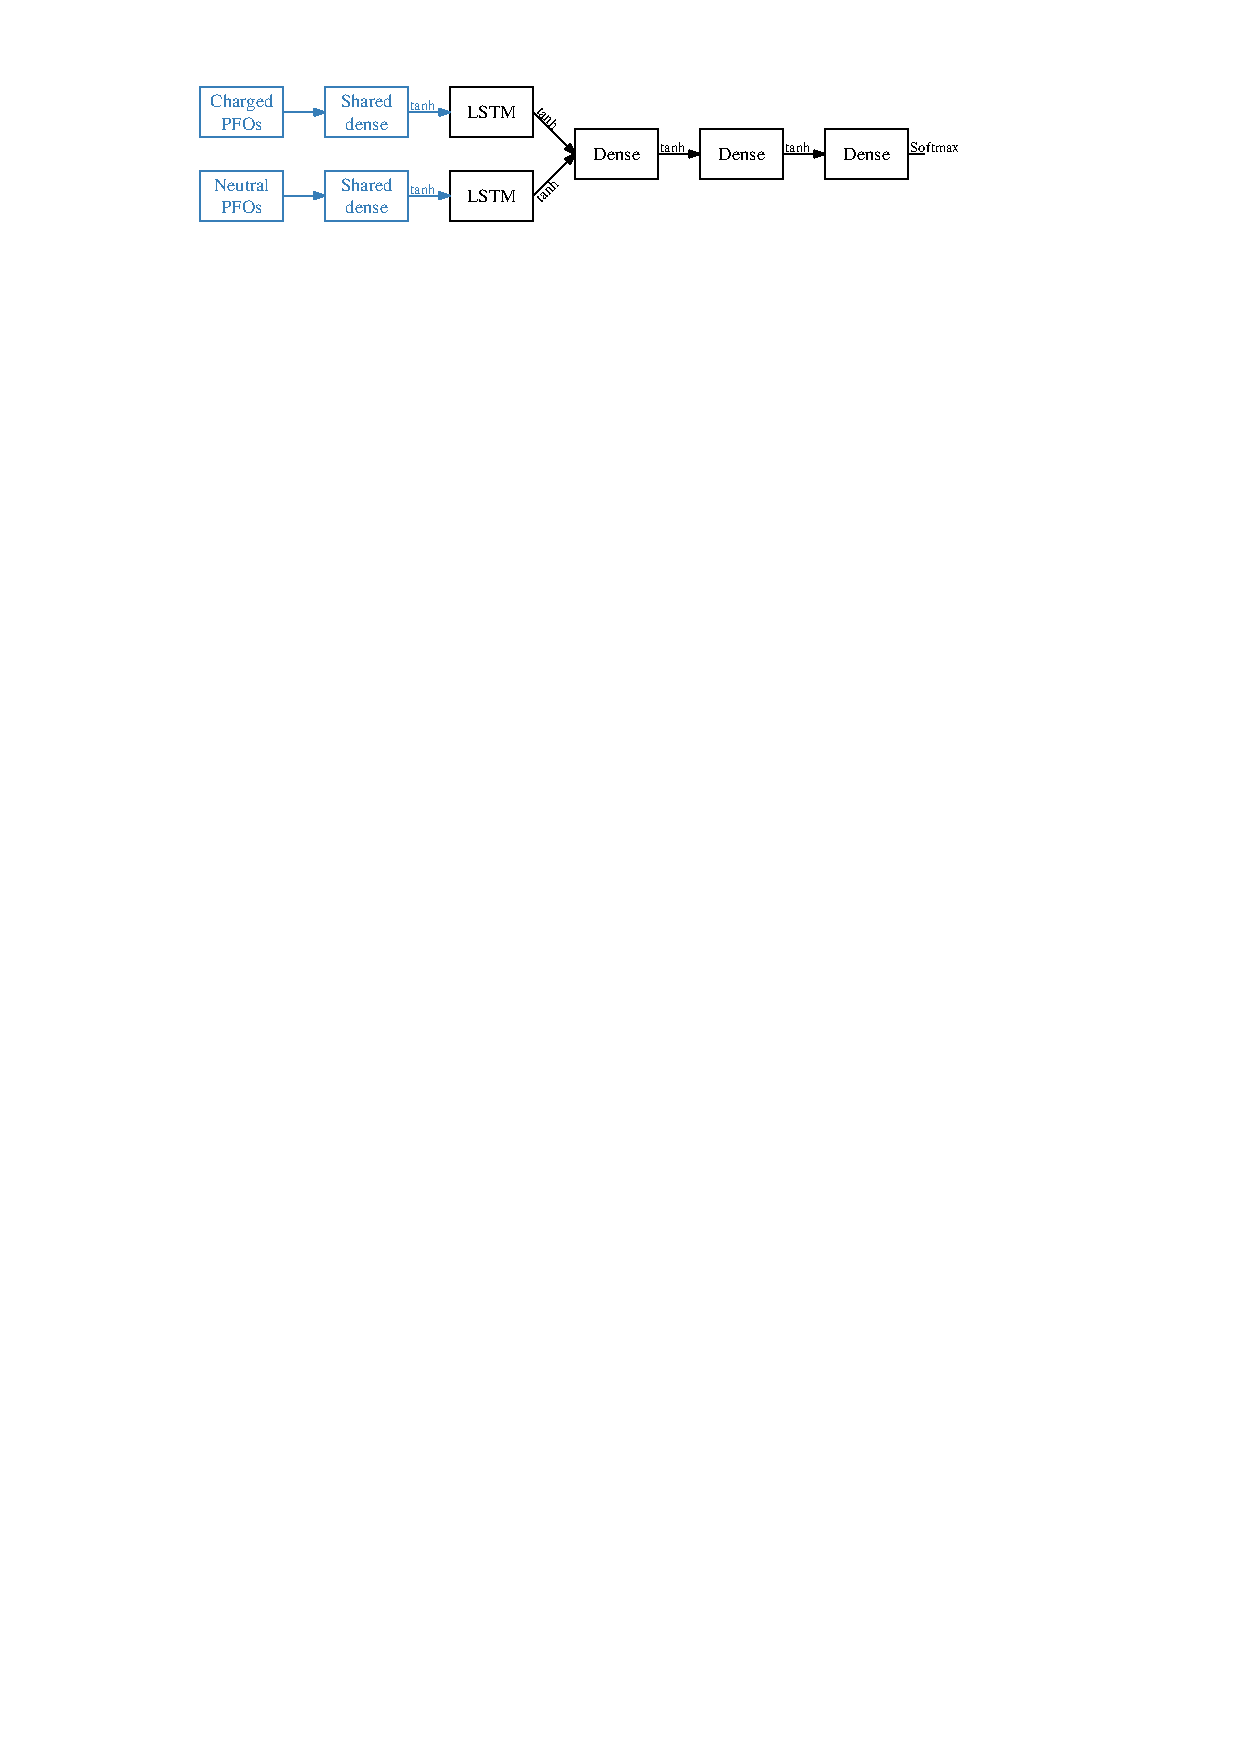
\includegraphics{./figures/decay_mode_classification/baseline_architecture.pdf}
  \caption{Architecture of the baseline model operating on sequences of charged
    and neutral PFOs. The activation function is denoted after each layer (cf.\
    Chapter~\ref{sec:ml}). Layers operating on sequential inputs are highlighted
    in blue.}
  \label{fig:pfo_rnn_baseline_arch}
\end{figure}

\subsection{Baseline Model}
\label{sec:pfo_baseline}

For training and evaluation of the model a sample of the
process~$\gamma^* \rightarrow \tau \tau \, \text{(hadr.)}$ is used (cf.\
Section~\ref{sec:bdt_eventsim}). Compared to the dataset used for the
tau identification studies, it features an updated tuning of the default decay
mode classification and an increase in the number of simulated events by
\SI{50}{\percent}. The sample is given in Appendix~\ref{app:mc16a_taus}.

In addition to the baseline tau selection given in
Section~\ref{sec:bdt_eventsim}, the visible transverse momentum of the hadronic
tau decay is required to be less than \SI{100}{\giga\electronvolt} at
reconstruction and generator-level. Moreover, only taus with the generated decay
mode being one of $h^\pm$, $h^\pm \pi^0$, $h^\pm \, {\geq} 2\pi^0$, $3h^\pm$ or
$3h^\pm \, {\geq} 1\pi^0$ and omitting decays containing
intermediate~\smash{$K^0$} are used. The mode composition of the sample
after applying this preselection is summarised in Table~\ref{tab:mode_reco_eff}.

\begin{table}[htb]
  \centering
  {\small\begin{tabular}{
  l
  S[table-format=2.2(2)]
  S[table-format=2.1(2)]
  S[table-format=2.1, round-mode=places, round-precision=1]
  S[table-format=2.1, round-mode=places, round-precision=1]
  }
  \toprule
  {Mode} & {$\mathcal{B}$ / \si{\percent}} & {$f_\text{BR}$ / \si{\percent}} & {$f_\text{reco}$ / \si{\percent}} & { $f_\text{reco+ID}$ / \si{\percent}} \\
  \midrule
  $h^\pm$ & 11.51 +- 0.05 & 18.3 +- 0.1 & 17.552988 & 21.365416 \\
  $h^\pm \pi^0$ & 25.93 +- 0.09 & 41.3 +- 0.2 & 41.854581 & 44.779216 \\
  $h^\pm \geq 2 \pi^0$ & 10.81 +- 0.09 & 17.2 +- 0.2 & 18.663134 & 15.775690 \\
  $3 h^\pm$ & 9.43 +- 0.05 & 15.1 +- 0.1 & 14.200414 & 13.315444 \\
  $3 h^\pm \geq 1 \pi^0$ & 5.09 +- 0.05 & 8.1 +- 0.1 & 7.728881 & 4.764232 \\
  \bottomrule
\end{tabular}

%%% Local Variables:
%%% mode: latex
%%% TeX-master: "../mythesis"
%%% End:
}
  \caption{Mode fractions of reconstructed \tauhadvis after the
    preselection~$f_\text{reco}$ and the expected mode fraction of a fully
    efficient reconstruction~$f_\text{BR}$ according to the branching
    ratio~$\mathcal{B}$.}
  \label{tab:mode_reco_eff}
  \todo[inline]{Better definitions for $f_\text{BR}$ and $f_\text{reco}$.}
\end{table}

The discrimination of the decay modes utilises kinematic quantities of the
reconstructed tau decay as well as the charged and neutral particle flow
objects. The variables attached to each neutral and charged PFO passed to the
network are summarised in the following:
\begin{description}
\item[Kinematic quantities of the reconstructed tau decay:] The visible
  transverse momentum~$p_\text{T}^\tau$ and the angular
  direction~$(\varphi_\tau, \eta_\tau)$ of the reconstructed tau axis. The
  momentum is calibrated at LC scale without applying any tau-specific energy
  calibrations.

\item[Kinematic quantities of charged and neutral PFOs:] The reconstructed
  transverse momentum $p_\text{T}^\text{PFO}$ and the signed angular distances
  to the reconstructed tau axis in transverse~$\Delta\varphi$ and longitudinal
  direction~$\Delta\eta \coloneqq \eta_\text{PFO} - \eta_\tau$. The transverse
  angular distance~$\Delta\varphi$ is defined analogously to the longitudinal
  case but also accounting for the periodicity in the azimuthal angle~$\varphi$.
  Angular deviations from the tau axis are used to ensure that coordinates are
  comparable between different tau candidates. \todo{Abbrev.\ angular distance
    -- should be explained for RNN-ID.}
\end{description}
For neutral PFOs the set of variables is extended to allow for the
identification of clusters originating from neutral pions. In addition to the
kinematic quantities, the following variables are used:
\begin{description}
\item[\smash{$\pi^0$}-identification score \smash{$S_\text{BDT}^{\pi^0}$}:]
  BDT-based discriminant combining shower shape information in the
  electromagnetic part of the calorimeter to identify neutral PFOs originating
  from photons of the \smash{$\pi^0$}-decay~\cite{atlas:taurec:decaymodes}.

\item[Total number of photons \smash{$N_\text{photons}^\text{tot}$}:] The total
  number of photons in all shots associated with a neutral PFO cluster (cf.\
  Section~\ref{sec:shot_reco}). Shots are associated with a cluster if it
  contains the seed cell of the shot, the PFO cluster fulfils
  $E_\text{T} > \SI{500}{\mega\electronvolt}$ and is within $\Delta R < 0.4$ to
  the tau axis. In cases where the cell is shared between multiple clusters, it
  is associated to the cluster to which the seed cell contributes with the
  largest weight~\cite{athena}.

  The fine segmentation of the strip layer in the EM calorimeter is used to
  count local energy maxima created by individual photons, allowing in some
  cases to recover the correct number of neutrals when the energy depositions of
  two neutral pions are reconstructed as a single cluster in the calorimeter.
  Moreover, it supports the identification of neutral pions as no shot
  information is used in the calculation of~\smash{$S_\text{BDT}^{\pi^0}$}.
\end{description}

Analogously to the RNN-based tau identification in Chapter~\ref{sec:rnn}, the
full dataset is split into training, validation and testing samples. The
transverse momenta of the reconstructed tau and PFOs are log-transformed and
subsequently standardised. For the neutral PFO specific
variables~\smash{$S_\text{BDT}^{\pi^0}$} and
\smash{$N_\text{photons}^\text{tot}$} no preprocessing is required. The
remaining kinematic variables, i.e.\ angular direction of the tau axis and
angular deviation of the PFO are scaled into the~$[-1, 1]$-interval.

Charged and neutral PFOs are passed in ascending transverse momentum ordering
\todo{why this ordering} to shared dense layers with 24 units each. A maximum of
three charged PFOs each corresponding to a \emph{charged} track and up to ten
neutral PFOs are used. The intermediate representations after the shared dense
layers are passed to the LSTM layers, each returning a vector of 24 activations.
The activations of both branches are merged and passed through a network of
three dense layers with 48, 32 and 5 units, respectively.

For a given reconstructed tau decay the model returns a probability for each of
the five decay modes. The decay mode is classified as the mode with the largest
probability estimate according to the model. A different scheme for determining
the decay mode would be to require the largest mode probability to exceed the
second largest by a predefined margin. This would increase the purity of the
classified modes at the expense of reducing the efficiency. As this scheme
depends on the requirements of the particular analysis, the following will focus
on classification according to the highest probability.

In contrast to the decay mode classification algorithm currently in use at the
ATLAS experiment, no discrimination of 1- and 3-prong modes according to the
number of reconstructed tracks that are classified as \emph{charged} is made.
However, as each charged PFO is associated with a \emph{charged} track the
number of tracks is indirectly available to the network. The network is not
strictly required to use this information allowing migrations of reconstructed
1-track (3-track) hadronic tau decays to 3-prong (1-prong) modes. If this
behaviour is not desired then the decay mode can be classified as the mode with
the highest probability that is compatible with the number of reconstructed
tracks. For the following studies these migrations are allowed. The loss in
classification power is small when constraining the model (a comparison is given
in Appendix~\ref{app:mode_classification_track_constraint}). \todo{see ben}

Neutral PFOs with small transverse momenta often do not originate from neutral
pions but from other sources. Moreover, it has not been studied how well they
are modelled in the simulation. Therefore, neutral PFOs passed to the network
(at training and evaluation time) are required to exceed a predefined
$p_\text{T}$-threshold. The diagonal efficiency, i.e.\ the fraction of correctly
classified modes in an independent sample, is summarised in
Table~\ref{tab:neut_ptcut} for four different $p_\text{T}$-thresholds. The
classification power does not degrade when no $p_\text{T}$-cut is applied,
indicating that the model is insensitive to low momentum PFOs from sources other
than a \smash{$\pi^0$}-decay. This is expected as the network has access to the
\smash{$\pi^0$}-identification score and transverse momentum. Additionally, only
a slow decrease in diagonal efficiency is observed when increasing the
threshold. The studies in this thesis use the \SI{1.5}{\giga\electronvolt}
threshold to account for potential mismodelling but further studies are needed
to prove the necessity of this cut.

\begin{table}[htb]
  \centering
  {\small\begin{tabular}{SS[table-format=2.2(2)]}%,table-space-text-post = \si{\meter}]}
  \toprule
  {$p_\text{T}$-cut / \si{\giga\electronvolt}} & {Diagonal efficiency / \si{\percent}} \\
  \midrule
  {--} & 78.43 \pm 0.06 \\
  1.0 & 78.09 \pm 0.08 \\
  1.5 & 77.95 \pm 0.04 \\
  2.0 & 77.88 \pm 0.06 \\
  2.5 & 77.54 \pm 0.04 \\
  \bottomrule
\end{tabular}

%%% Local Variables:
%%% mode: latex
%%% TeX-master: "../mythesis"
%%% End:
}
  \caption{Diagonal efficiency evaluated on the validation sample as a function
    of the transverse momentum threshold for neutral PFOs. The network is
    retrained for each threshold.}
  \label{tab:neut_ptcut}
\end{table}

Figure~\ref{fig:mode_proba_ptcut} depicts two examples of mode probability
estimates on the testing sample. A complete set of probabilities for all five
decay modes is omitted for brevity and can be found in
Appendix~\ref{app:baseline_probabilities}. The $h^\pm$~mode probability in
Figure~\ref{fig:1p0n_proba} shows that the estimated probabilities for generated
modes containing one or more neutral pions are frequently small. Nevertheless,
when no neutral PFOs are reconstructed they can be as large as
\SI{90}{\percent}, causing decays to be falsely classified. The same feature can
be observed in Figure~\ref{fig:1p1n_proba}, where the $h^\pm \pi^0$ mode
probabilities are small. Additionally, generated 1-prong decays with more than
one neutral pion often exceed $h^\pm \pi^0$ probabilities of \SI{50}{\percent}
leading to significant migrations of true $h^\pm \, {\geq} 2 \pi^0$ to the
$h^\pm \pi^0$ decay mode.

\begin{figure}[htb]
  \begin{subfigure}[t]{0.48\textwidth}
    \centering
    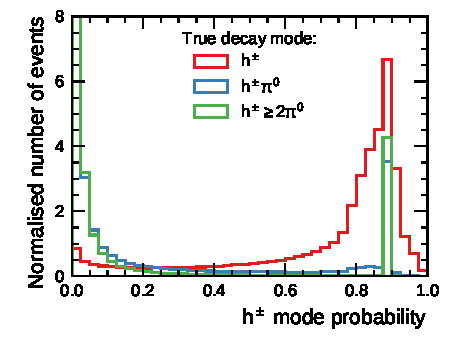
\includegraphics{./figures/decay_mode_classification/mode_proba_baseline_ptcut_1_5_only_1p/proba_1p0n.pdf}
    \vspace*{-1.6em}
    \label{fig:1p0n_proba}
  \end{subfigure}\hfill
  \begin{subfigure}[t]{0.48\textwidth}
    \centering
    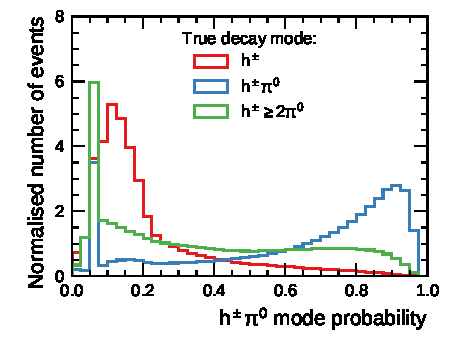
\includegraphics{./figures/decay_mode_classification/mode_proba_baseline_ptcut_1_5_only_1p/proba_1p1n.pdf}
    \vspace*{-1.6em}
    \label{fig:1p1n_proba}
  \end{subfigure}
  \caption{Mode probabilities for the $h^\pm$ and $h^\pm \pi^0$ modes estimated
    by the RNN for a given true decay mode. Modes with three charged hadrons
    have small $h^\pm$ and $h^\pm \pi^0$ probabilities and are omitted for
    clarity.}
  \label{fig:mode_proba_ptcut}
\end{figure}

The migration probability of generated decay modes to a given reconstructed mode
can be summarised in the so called \emph{migration matrix}.
Figure~\ref{fig:migmat_comparison_baseline_15cut} shows migration matrices of
the ATLAS default algorithm~\cite{atlas:taurec:decaymodes} and the RNN-based
decay mode classification. The diagonal entries give the efficiencies to
correctly reconstruct the corresponding decay mode, while the off-diagonal
measures the migration probability between modes. The diagonal efficiency can
also be interpreted as the mean of the diagonal entries of this matrix weighted
by the mode fractions (cf.\ Table~\ref{tab:mode_reco_eff}). The individual
efficiencies and migration probabilities in the matrix can vary between
different trainings of the network as a decrease in efficiency in one mode can
be compensated by an improvement in another. Nevertheless, the diagonal
efficiency is a stable metric between different trainings and is used as a
figure of merit for subsequent investigations.

\begin{figure}[htb]
  \begin{subfigure}[t]{0.48\textwidth}
    \centering
    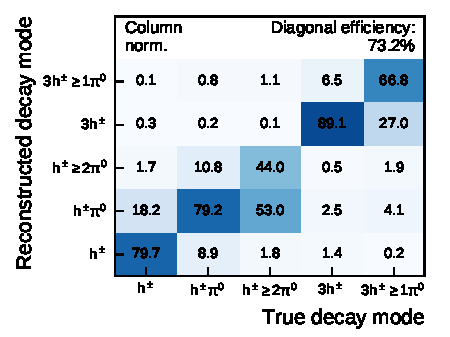
\includegraphics{./figures/decay_mode_classification/mig_mat_pantau.pdf}
    \subcaption{ATLAS default algorithm: \emph{PanTau}}
  \end{subfigure}\hfill
  \begin{subfigure}[t]{0.48\textwidth}
    \centering
    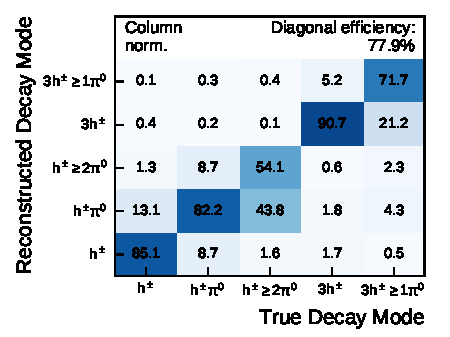
\includegraphics{./figures/decay_mode_classification/mig_mat_baseline_ptcut_1_5.pdf}
    \subcaption{RNN with neutral PFO $p_{\text{T}}$-cut of
      \SI{1.5}{\GeV}}
  \end{subfigure}
  \caption{Migration matrices showing the migration probabilities of the true
    decay modes to the reconstructed modes in \si{\percent}. Evaluation on the
    independent testing sample. Statistical fluctuations due to limited sample
    size can be neglected.}
  \label{fig:migmat_comparison_baseline_15cut}
\end{figure}

In comparison with the ATLAS default algorithm, the RNN-based decay mode
classification improves the efficiencies of all five decay modes leading to an
absolute increase in diagonal efficiency of \SI{4.8}{\percent} to a total of
\SI{78.0}{\percent}. This corresponds to a reduction in the number of
misclassified \tauhadvis of \SI{18}{\percent}. Furthermore, a significant
reduction in migrations due to under- or overestimation of the number of neutral
pions is observed. Migrations between 1- and 3-prong modes are of similar
magnitude for both algorithms.

Due to the reduction of migrations between different modes an overall
improvement in purity of the reconstructed modes is expected. This is shown in
the so called \emph{purity matrix} in
Figure~\ref{fig:puritymat_comparison_baseline_15cut}, where each row gives the
fractional composition of the reconstructed decay modes in terms of the
generated mode. The comparison shows the expected improvement in purity of all
five reconstructed modes. A more detailed discussion of the results will be
given after extending the model with additional information.

\begin{figure}[htb]
  \begin{subfigure}[t]{0.48\textwidth}
    \centering
    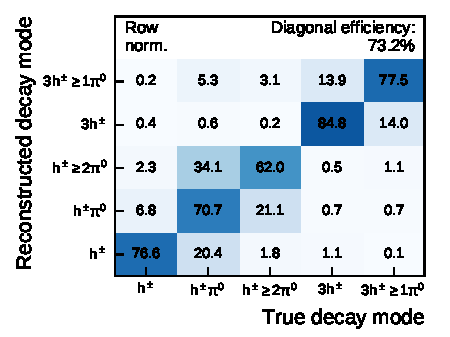
\includegraphics{./figures/decay_mode_classification/comp_mat_pantau.pdf}
    \subcaption{ATLAS default algorithm: \emph{PanTau}}
  \end{subfigure}\hfill
  \begin{subfigure}[t]{0.48\textwidth}
    \centering
    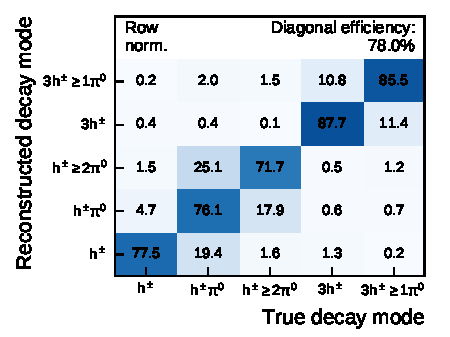
\includegraphics{./figures/decay_mode_classification/comp_mat_baseline_ptcut_1_5.pdf}
    \subcaption{RNN with neutral PFO $p_{\text{T}}$-cut of
      \SI{1.5}{\giga\electronvolt}}
  \end{subfigure}
  \caption{Purity matrices showing the fractional composition of the
    reconstructed decay modes in \si{\percent}. Evaluation on the independent
    testing sample. Statistical fluctuations due to limited sample size can be
    neglected.}
  \label{fig:puritymat_comparison_baseline_15cut}
\end{figure}

\subsection{Additional Information}
\label{sec:add_info}

This section aims to increase the discrimination power of the RNN-based decay
mode classification by including additional information into the network. The
focus lies on the inclusion of conversion tracks, shots, and further properties
of the neutral PFO clusters. The following describes the intention behind each
source of additional information and how it is included into the network
architecture.

\subsubsection{Conversion Tracks}
Often photons from the \smash{$\pi^0$}-decay convert in the material of the
inner detector into electron--positron pairs. The magnetic field bends the pair
from the direction of the initiating photon, spreading out the energy deposition
in the EM calorimeter. This can lead to neutral PFOs being reconstructed from
clusters originating from individual electrons, affecting the
\smash{$\pi^0$}-identification score and the number of associated shots. In some
cases the algorithm can fail to reconstruct neutral PFOs, thus the presence of
conversion tracks can be an indicator of decay modes containing neutral pions.
The inclusion of conversion tracks in the classification aims to reduce
migrations to decay modes with fewer neutrals.

The architecture of the baseline model (cf.\
Figure~\ref{fig:pfo_rnn_baseline_arch}) is extended by a third branch taking a
sequence of tracks classified as \emph{conversion} according to the track
classification algorithm. Its sequence of layers is identical to the other
branches except that the number of units in the shared dense and LSTM layers are
reduced to 16 (from 24). To account for the increased number of units of the
three merged branches, the size of the consecutive dense layers are increased to
64 and 32 units (from 48/32).

A maximum of four conversion tracks are passed to the network in ascending
transverse momentum ordering. Tracks are required to pass a transverse momentum
threshold of \SI{400}{\MeV} from the track reconstruction. The inputs for each
track contain the transverse momentum of the track~$p_\text{T}^\text{track}$,
the angular direction of the tau axis~$(\varphi_\tau, \eta_\tau)$ and the
angular distance~$(\Delta\varphi, \Delta\eta)$ between track and tau axis. The
angular distances are calculated using track parameters at the perigee with
respect to the beamspot and alternatively using the position of the extrapolated
track hit on the face of EM1.

\subsubsection{Shots}

The boosted topology of tau decays in ATLAS can cause neutral pion clusters to
merge with clusters originating from other pions. Using purely kinematic
quantities of reconstructed PFOs does not allow to identify merged neutral pion
clusters, which may lead to an underestimation of the number of neutrals. The
baseline model already includes the number of photons in shots matched to a
given neutral PFO~$N_\text{photons}$, significantly improving the discrimination
power of the network and accounting for an absolute \SI{1.5}{\percent} of
diagonal efficiency. The network is extended to receive a sequence of shots
associated with a reconstructed tau decay. This differs from the approach in the
baseline model by also including transverse momentum and the angular position of
shots in the calorimeter.

The network architecture is identical to the one used for conversion tracks in
the previous section. Analogously, up to six reconstructed shots are passed to
the network in ascending transverse momentum ordering. Only shots with one or
more photons~$N_\text{photons} > 0$ are considered (cf.\
Section~\ref{sec:shot_reco}). This selection applies a lower threshold on the
transverse momentum~\smash{$p_\text{T}^\text{shot}$} to suppress shots
originating from noise or fluctuations of the photon
shower~\cite{atlas:taurec:decaymodes}.
% Shots from the transition region of the calorimeter~$1.37 < |\eta| < 1.52$ are
% not used.
The set of input variables is defined in analogy to charged PFOs and conversion
tracks by replacing the inputs with the corresponding shot quantities.

\subsubsection{Neutral PFO Cluster Properties}

Further improvements in classifying events with merged clusters can be achieved
by employing shower shape information. For this clusters created during PFO
reconstruction (cf.\ Section~\ref{sec:tau_pflow}) are used to calculate moments
and other cluster properties.
% Clustering in Presampler, EM1 and EM2
The discriminants are summarised in Table~\ref{tab:cluster_variables} and
include variables also used for $\pi^0$-identification.

\begin{table}[htb]
  \centering
  {\def\arraystretch{1.4}\small
  \begin{tabular}{p{4.5cm}p{9cm}}
    \toprule
    \textbf{Lateral shower width}\newline$\langle R^2 \rangle$ &
    Second moment of the radial distance $R$ between cluster cells and shower axis \cite{atlas_topoclustering}. \\

    \textbf{$\eta$-width in EM1}\newline$\langle (\eta - \eta_\text{cluster})^2\rangle$ &
    Second moment of the pseudorapidity distance between cluster cells in EM1
    and the energy barycentre of the cluster~$\eta_\text{cluster}$~\cite{atlas:taurec:decaymodes}. \\

    \textbf{Number of pos.\ cells in EM1} $N_\text{EM1}^\text{pos}$ &
    Number of cells with positive energy in EM1~\cite{atlas:taurec:decaymodes}.\\

    \textbf{Core energy fraction}\newline$f_\text{core}$ &
    Fraction of the total cluster energy contained in the highest energetic cell
    in Presampler, EM1 and EM2~\cite{atlas_topoclustering}. \\

    \textbf{Energy fraction in EM2}\newline$f_\text{EM2}$ &
    Fraction of energy contained in EM2.\\
    \bottomrule
  \end{tabular}
  }
  \caption{Variables derived from properties of neutral PFO clusters.}
  \label{tab:cluster_variables}
\end{table}

Variables describing the longitudinal shower shape, e.g.\ the depth of the
shower centre~$\lambda_\text{centre}$ or longitudinal
spread~$\langle \lambda^2 \rangle$, are not found to improve decay mode
classification. Only the energy fraction in the EM2 sampling of the calorimeter
is used as it is highly anti-correlated with the fraction in EM1, thus not
providing additional separation power. Additionally, a variable measuring the
overlap of neutral and charged PFOs is examined separately from the variables in
Table~\ref{tab:cluster_variables}. It is the fraction of transverse momentum
subtracted from the cluster during PFO reconstruction
\begin{align*}
  f_\text{sub} = \frac{p_\text{T}^\text{cluster} - p_\text{T}^\text{neut.\ PFO}}{p_\text{T}^\text{cluster}} \eqcomma
\end{align*}
where~$p_\text{T}^\text{cluster}$ is the transverse momentum of the PFO cluster
and $p_\text{T}^\text{neut.\ PFO}$ the transverse momentum of the neutral PFO,
i.e.\ after subtracting the energy of charged hadrons. The neutral PFO input
variables are extended using these properties, therefore not requiring changes
in network architecture.

\subsubsection{Performance Evaluation}

Table~\ref{tab:pfo_add_experiments} summarises the diagonal efficiency of the
RNN-based classification for the different experiments. In addition to the
previously described inputs, the performance after including hadronic PFOs,
i.e.\ objects created from energy in the hadronic part of \emph{TopoClusters} in
the core region~$\Delta R < 0.2$ of the reconstructed tau, is evaluated. It is
not found to significantly improve the performance considering the increase in
model complexity. Moreover, a model using an ascending $\pi^0$-identification
score ordering for the neutral PFOs shows no significant improvement over the
transverse momentum ordering.

\begin{table}[htb]
  \centering
  {\small\begin{tabular}{p{5cm}S[table-format=1.4(4)]S[table-format=2.2(2)]S[table-format=1.2(2)]}
  \toprule
  {Experiment} & {Loss} & {Diag.\ eff.\ / \si{\percent}} & {Diag.\ eff.\ gain (abs.) / \si{\percent}} \\
  \midrule
  Conversion tracks & 0.5186 +- 0.0013 & 79.40 +- 0.07 & 1.45 +- 0.08 \\
  Conversion tracks (extrapol.) & 0.5224 +- 0.0012 & 79.23 +- 0.06 & 1.28 +- 0.07 \\
  Shots & 0.5239 +- 0.0011 & 79.52 +- 0.06 &  1.57 +- 0.07 \\
  Neut.\ PFO cluster properties & 0.5310 +- 0.0010 & 79.07 +- 0.06 & 1.12 +- 0.07 \\
  Hadronic PFOs & 0.5433 +- 0.0007 & 78.30 +- 0.04 & 0.35 +- 0.06 \\
  Fraction of subtracted $p_\text{T}$ & 0.5466 +- 0.0005 & 78.26 +- 0.03 & 0.31 +- 0.05 \\
  $\pi^0$-BDT ordering & 0.5511 +- 0.0013 & 78.01 +- 0.07 & 0.06 +-0.08 \\
  \bottomrule
\end{tabular}

%%% Local Variables:
%%% mode: latex
%%% TeX-master: "../mythesis"
%%% End:
}
  \caption{Decay mode classification performance after extending the RNN. The
    metrics are evaluated on the validation sample.}
  \label{tab:pfo_add_experiments}
\end{table}

The largest improvements in diagonal efficiency are observed when including
conversion tracks and shots in the classification. Both reduce migrations to
modes with fewer neutral pions, while minimally increasing the probability of
overestimating the neutral pion count in some modes. Moreover, using the
extrapolated track position does not show an improvement over using the track
parameters at the perigee with respect to the beamspot.
% This is likely due to parameters at the beamspot more closely resembling the
% original direction of the photon Migration and purity matrices for the
% different experiments are omitted for brevity and can be found in
% Appendix~\ref{sec:app_decay_mode_exp} \todo{Remove from appendix -- not
% interesting?}.

A significant improvement in classification accuracy of \SI{1.12 +-
  0.07}{\percent} is observed, when extending the neutral PFO variable set with
additional cluster properties. Furthermore, the fraction of transverse momentum
subtracted from the cluster~$f_\text{sub}$ significantly improves the
classification power at a minimal complexity cost. A possible future extension
of the network would be to include the $\pi^0$-identification variables in each
neutral PFO, thus allowing the network to learn a $\pi^0$-identification
specialised for decay mode classification.

Finally, alternative architectures including bidirectional LSTM and multiple
consecutive LSTM layers are tested, only showing marginal improvements in the
range of \num{0.2} to \SI{0.3}{\percent} in diagonal efficiency over a model
using a single LSTM layer.

\subsection{Extended Model}
\label{sec:extended_model}

The baseline model is extended using multiple sources of additional information
from the previous section. This includes conversion tracks (without track
extrapolation), shots and additional properties of neutral PFO clusters
including the fraction of subtracted transverse momentum. The architecture
% \footnote{Shared dense/LSTM layers: 24 units (chrg.\ \& neut.\ PFOs), 16 units
% (conv.\ tracks and shots). Dense layers: 64/32/5 units.}
is adjusted accordingly to allow sequences of conversion tracks and shots to be
passed to the network. The same \SI{1.5}{\GeV} transverse momentum threshold is
applied to neutral PFOs.

After extending the model, the peaks in the estimated mode probabilities for tau
decays without reconstructed neutral PFOs (cf.\
Figure~\ref{fig:mode_proba_ptcut}) are significantly reduced as the additional
conversion track and shot information can aid in the discrimination even when no
neutral PFOs are present. For completeness plots of the mode probability
estimates of the extended model are summarised in
Appendix~\ref{app:combined_probabilities}.

In Figure~\ref{fig:decay_mode_combined} the migration and purity matrices of the
extended model are shown. The additional discrimination power increases the
diagonal efficiency from~\SI{78.0}{\percent} of the baseline model
to~\SI{81.5}{\percent}. This is due to an absolute increase in efficiency of the
order of~\SI{5}{\percent} for modes containing one or more neutral pions. The
improvement in diagonal efficiency corresponds to a decrease in the number of
misclassified \tauhadvis by \SI{31}{\percent} with respect to the default
algorithm.
% $h^\pm \pi^0$, $h^\pm \geq 2\pi^0$ and $3h^\pm\geq1\pi^0$.
The purity is mostly affected in the $h^\pm$ and $h^\pm \, {\geq} 2\pi^0$~modes
with an absolute purity improvement of~\SI{4.9}{\percent} and~\SI{7.0}{\percent}
over the baseline model. For the reconstructed $h^\pm$~mode the large
contamination due to the abundant $h^\pm \pi^0$~mode is mainly reduced by the
inclusion of conversion tracks and shots.
% Tau decays without reco. neutral PFOs!
Moreover, the reconstructed $h^\pm \, {\geq} 2\pi^0$~mode purity, also showing
contamination of $h^\pm \pi^0$, is primarily improved by the inclusion of shot
information.
% Merged pi0 clusters

\begin{figure}[htb]
  \begin{subfigure}{0.48\textwidth}
    \centering
    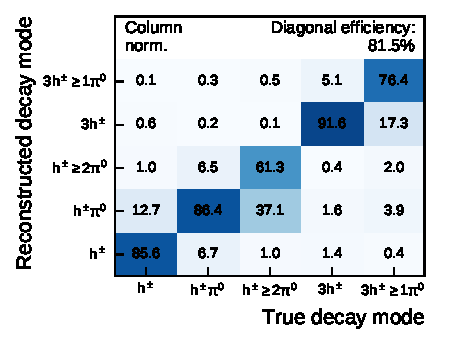
\includegraphics{./figures/decay_mode_classification/combined_sub_e_moments_shots_conv_ptcut_1_5/mig_mat.pdf}
    \subcaption{Migration matrix}
  \end{subfigure}\hfill
  \begin{subfigure}{0.48\textwidth}
    \centering
    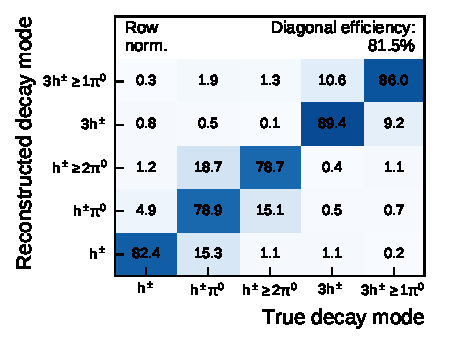
\includegraphics{./figures/decay_mode_classification/combined_sub_e_moments_shots_conv_ptcut_1_5/comp_mat.pdf}
    \subcaption{Purity matrix}
  \end{subfigure}
  \caption{Migration and purity matrix of the extended model including
    conversion, shot and additional cluster information. Evaluated on the
    testing sample with negligible statistical errors.}
  \label{fig:decay_mode_combined}
\end{figure}

The dependency of the mode classification efficiency and purity on the
reconstructed transverse momentum of the tau lepton is shown in
Figure~\ref{fig:mode_efficiency_purity}. The efficiencies of the $h^\pm$,
$h^\pm \pi^0$ and $3h^\pm$ modes show no strong dependence on the transverse
momentum of the tau. In contrast to this, the 1-prong mode with more than one
and the 3-prong mode with neutral pions show a significant increase in
efficiency over the \num{20} to \SI{40}{\GeV} transverse momentum range. A
possible explanation is that the classifier misses increasingly soft neutral
pions for low momentum tau decays. Therefore, migrations are reduced at higher
transverse momenta leading to an increase in purity in all five decay modes.

\begin{figure}[htb]
  \begin{subfigure}{0.48\textwidth}
    \centering
    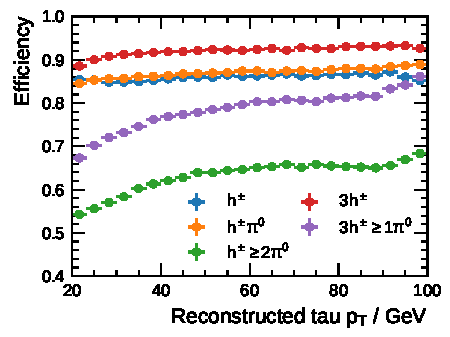
\includegraphics{./figures/decay_mode_classification/combined_sub_e_moments_shots_conv_ptcut_1_5/efficiency_profile.pdf}
    \vspace*{-1.6em}
    \subcaption{}
  \end{subfigure}\hfill
  \begin{subfigure}{0.48\textwidth}
    \centering
    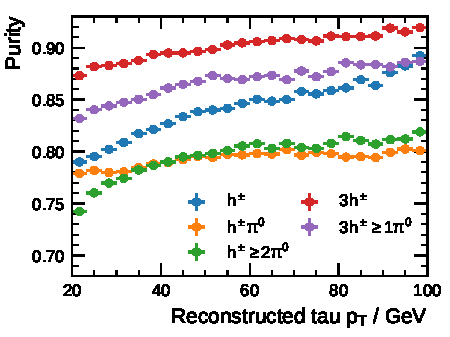
\includegraphics{./figures/decay_mode_classification/combined_sub_e_moments_shots_conv_ptcut_1_5/purity_profile.pdf}
    \vspace*{-1.6em}
    \subcaption{}
  \end{subfigure}
  \caption{Efficiency and purity profiles of the decay mode classification using
    the extended model. Evaluated on the testing sample. Statistical errors are
    not visible as they are of the order of the marker size.}
  \label{fig:mode_efficiency_purity}
\end{figure}

The efficiency and purity profiles in Figure~\ref{fig:mode_efficiency_purity}
indicate that the RNN-based classification algorithm could be used beyond the
$\SI{\sim 100}{\GeV}$ design limit of the particle flow algorithm, as the
efficiencies and purities remain flat at large transverse momenta.
Figure~\ref{fig:mode_efficiency_purity_highpt} shows the profiles after
retraining the model on data without applying an upper limit on the
reconstructed transverse momentum of the tau. The mode efficiencies and purities
reach a maximum at transverse momenta of approximately \SI{100}{\GeV}, after
which, with exception of the $h^\pm \, {\geq} 2 \pi^0$ mode, the performance
declines slowly.
% Increased boost leads to 1pXn merges
This shows that the transverse momentum range of the classification could be
extended to approximately \SI{200}{\GeV}, while still keeping the performance
characteristics comparable to the performance at \SI{20}{\GeV}. The diagonal
efficiency at transverse momenta below \SI{100}{\GeV} is \SI{81.4}{\percent} and
unaffected by the training on the extended momentum range, while at higher
momenta it amounts to \SI{77.6}{\percent}. The extended momentum range could be
beneficial to analyses with high-momentum taus that also employ decay mode
information. \todo{Explain what happens at large transverse momenta}

\begin{figure}[htb]
  \begin{subfigure}{0.48\textwidth}
    \centering
    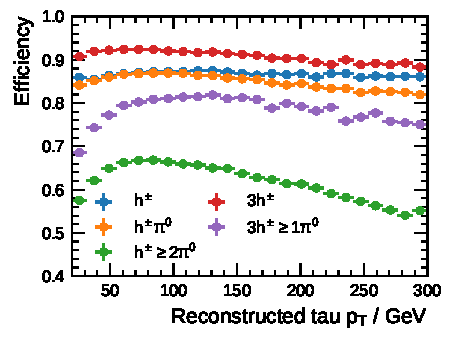
\includegraphics{./figures/decay_mode_classification/highpt/efficiency_profile_extended.pdf}
    \vspace*{-1.6em}
    \subcaption{}
  \end{subfigure}\hfill
  \begin{subfigure}{0.48\textwidth}
    \centering
    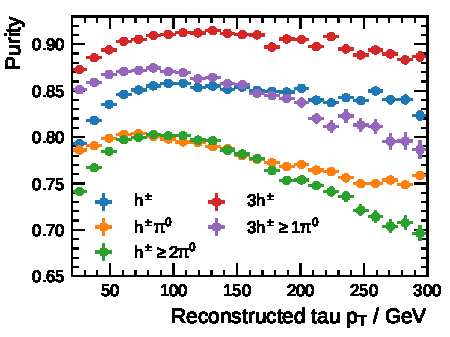
\includegraphics{./figures/decay_mode_classification/highpt/purity_profile_extended.pdf}
    \vspace*{-1.6em}
    \subcaption{}
  \end{subfigure}
  \caption{Efficiency and purity profile of the decay mode classification using
    the extended model trained on the full transverse momentum range of the
    sample. Evaluated on the testing sample.}
  \label{fig:mode_efficiency_purity_highpt}
\end{figure}

In the ATLAS experiment two alternative energy calibrations for reconstructed
hadronic tau decays are available. These use the reconstructed decay mode to
increase the resolution of the visible transverse momentum measurement. The
improvement in classification accuracy when using the RNN can therefore lead to
a better energy resolution, when one of these calibrations is used.

A different application of the RNN-based decay mode classification would be for
the determination of the $\mathcal{CP}$ nature of the Higgs boson, which can
measured using various decay modes of the tau lepton in~$H \to \tau + \tau$
events~\cite{Berge2014}. An example is the
double~$\tau \to \rho + \nu_\tau \to \pi + \pi^0 + \nu_\tau$ decay,
corresponding to the $h^\pm \pi^0$ mode. The $\mathcal{CP}$ measurement requires
the neutral pions in the final state to be reconstructed and identified.
However, the RNN-based classification does not provide a direct causal
relationship between a neutral PFO and the decay mode decision. Therefore, an
additional algorithm would be required to identify and reconstruct neutral pions
in an event of a given decay mode. For the $\mathcal{CP}$ measurement in the
$\rho\nu$ mode using the extended model an absolute improvement in mode
efficiency of~\SI{7.2}{\percent} and purity of~\SI{8.2}{\percent} is expected
for a single tau. Depending on the effectiveness of reconstructing the neutral
pions this could lead to a significant improvement in the signal to background
ratio for Higgs-$\mathcal{CP}$ analyses. The remaining modes show similar
improvements in efficiency and purity with respect to the algorithm currently in
use at the ATLAS experiment.

%%% Local Variables:
%%% mode: latex
%%% TeX-master: "mythesis"
%%% End:
